\documentclass[11pt,a4paper]{report}
\usepackage[utf8]{inputenc}
\usepackage[T1]{fontenc}
\usepackage[english, french]{babel} %français
\usepackage{amsmath}
\usepackage{amsfonts}
%\usepackage{amssymb}
\usepackage{makeidx}
\usepackage{graphicx}
\usepackage[left=2cm,right=2cm,top=2cm,bottom=2cm]{geometry}
\usepackage{stmaryrd} % parallel symbol
\usepackage{mathrsfs} % curly D symbol
\usepackage{dsfont} % hollow Z, R, N symbols
\usepackage[colorlinks=true, linkcolor=black, citecolor=black]{hyperref} % hyperlinks

\usepackage{eso-pic}
\newcommand\BackgroundPic{
\put(0,0){
\parbox[b][\paperheight]{\paperwidth}{%
\vfill
\centering
\includegraphics[width=\paperwidth,height=\paperheight,
keepaspectratio]{img/cover/cover_img.png}%
\vfill
}}}

% Code
\usepackage{listings}
\lstloadlanguages{[5.2]Mathematica}

% citations	
\usepackage{epigraph}
\setlength\epigraphwidth{12cm}

% subfigure
\usepackage{caption}
\usepackage{subcaption} 

% hyperlinks
%\usepackage{hyperref}
\usepackage{url}



%% user-defined commands 
\newcommand\Chapter[2]{
  \chapter[#1: {\itshape#2}]{#1\\[2ex]\Large\itshape#2}
}

\newcommand{\tr}[1]{\ensuremath{ \text{tr}\left(#1\right) }}
\newcommand{\atpt}[1]{\ensuremath{ \Big|_{\text{#1}} }}
\newcommand{\funcd}[1]{\ensuremath{\frac{\delta}{\delta #1}}}
\newcommand{\p}[1]{\partial_{#1}}
\newcommand{\derivh}[2]{\ensuremath{\frac{d^{#2}}{d #1^{#2}}}}
\newcommand{\deriv}[1]{\ensuremath{\frac{d}{d #1}}}
\newcommand{\gam}{\ensuremath{\Gamma}} % shortcut for the uppercase gamma letter used everywhere
\newcommand{\gamleg}{\ensuremath{\Gamma_k^{\text{Leg}}}} % Legendre effective action at scale k
\newcommand{\gamlegtwo}{\ensuremath{\Gamma_k^{\text{Leg }(2)}}}
\newcommand{\fdot}{\ensuremath{~\cdot~}} % point dans les déf de fonctions

% the triple equal sign I use to define something
\newcommand{\define}{\ensuremath{ \overset{\text{def}}{=} }}

% curly functional measure sign
\newcommand{\D}{\ensuremath{ \mathscr{D} }}

\begin{document}
 

\begin{titlepage}

\selectlanguage{english}
\thispagestyle{empty}



\begin{center}
\vspace{1.3cm}
{M1 de Physique
Fondamentale et Magistère 2}\\
\vspace{0.8cm}
{\Large{Internship from the 22nd of April to the 22nd of July, 2013}\\at the Manchester Centre for Nonlinear Dynamics, the University of Manchester.}\\ 
\end{center}
\vspace{1.5cm}
\begin{center}
\rule{\textwidth}{1mm}
\Huge{\Huge \textbf{Particle size segregation in granular free-surface flows}} 
\rule[0.3cm]{\textwidth}{1mm}\\
\end{center}

\vspace{0.7cm}
\begin{tabular}{lll}
~\\
~\\
~\\
~\\
~\\
~\\
~\\
~\\
~\\
~\\
~\\
~\\
~\\
~\\
~\\
~\\
~\\
~\\
~\\
~\\
~\\
~\\
~\\
~\\
~\\
~\\
~\\
~\\
~
\end{tabular}
\begin{center}
\Large{\textbf{Intern:} Nicolas Macé}\\
\Large{\textbf{Internship supervisor:} Nico Gray}\\
\end{center}

\end{titlepage}
\pagebreak 
\selectlanguage{english}
\begin{abstract}
In granular flows, large particles tend to go at the flow surface, while small particles tend to go at the flow base.
This particle size segregation is still poorly understood, especially in natural debris flows, where this effect is combined with strong sheer rates to cause lateral levees formation and flow channelisation. 

We seek to model and understand the properties of such granular flows.
We base our analysis on large-scale granular chute experiments conducted in 2011 \cite{main}.
We model the two-dimensional flow in the centre plane of the avalanche, and we propose and explanation for the observed structure. 
We develop a code to model the whole three-dimensional flow.

\selectlanguage{french}
\begin{center}
\textbf{Résumé}
\end{center}
Dans les écoulements granulaires, les grains les plus gros ont tendance à monter vers la surface, tandis que les grains les plus petits ont tendance à couler vers la base.
Cette ségrégation en milieu granulaire est encore mal comprise, particulièrement dans les laves torrentielles, dans lesquelles la combinaison de la ségrégation et du taux de cisaillement important de l'écoulement donne lieu à la formation de bourrelets latéraux canalisant ce dernier.

Nous cherchons à modéliser et à comprendre les propriétés de ces écoulements granulaires.
Nous basons notre analyse sur des expériences de grande taille conduites en 2011 \cite{main}. 
Nous modélisons l'écoulement bidimensionnel du plan centre de l'avalanche, et nous avançons une explication de la structure observée.
Nous développons un code modélisant l'écoulement tridimensionnel entier.
\end{abstract}

\selectlanguage{english}

\pagebreak

\begin{center}
\Huge \textbf{Particle size segregation in granular free-surface flows}
\end{center}


\section*{\Huge{Introduction}}

The Manchester Centre for Nonlinear Dynamics of the University of Manchester is group of researchers studying nonlinear phenomena.
The research notably includes turbulence and bifurcation in fluid dynamics, shock formation and segregation in granular materials.
Approximately 25 researchers, with physics or applied mathematics backgrounds are working inside the group. 

In nonlinear dynamics, very few theoretical results are available, and the interplay between experiments, theories and  simulations is of paramount importance. 
For example, granular media researchers, though primarily focused on theoretical modelling and computation, are also actively developing three experiments housed in the neighbouring physics building.

During my internship I studied a very specific topic: segregation in granular flows. 
But since I had no knowledge on granular materials at all when I arrived, I first took interest in understanding what is a granular material, and how we can model and understand it. \\

The first chapter of the internship report is thus a very general introduction to granular materials and granular flows. At the end of this chapter, we give qualitative ideas about the segregation effect, ideas which are developed more rigorously in the appendix.

The second chapter will focus more specifically on the experiment we seek to model and understand, and on the approach we took to model it.

The third chapter give our results and discuss them.


%\maketitle
\tableofcontents
 

\chapter{The Lifshitz model: general presentation.}

\section{The Lifshitz model and its main features}

\subsection{The Lifshitz model}

\subsubsection{The modulated phase and the Lifshitz phase diagram.}

The Lifshitz model aims at describing a number of physical many-body systems. They share a common intriguing feature: having a so called modulated - or stripped - phase (fig. \eqref{fig:evol_strip}). In this phase, the order parameter is spatially periodic in one or several directions of space. We will label with a $\sslash$ sign quantities living in these directions, and $\perp$ the quantities living in the orthogonal subspace.

Typically, the phase diagram of such a physical system will resemble the one presented in fig. \eqref{fig:phase_diagram}.

\begin{figure}[htp]
\centering
\begin{subfigure}{.33\textwidth}
	\centering
	\includegraphics[width=.9\linewidth]{img/chap1/sol_Lif_t20.png}
	\caption{}
	\label{lif_t20}
	\end{subfigure}%
\begin{subfigure}{.33\textwidth}
	\centering
	\includegraphics[width=.9\linewidth]{img/chap1/sol_Lif_t60.png}
	\caption{}
	\label{lif_t60}
\end{subfigure}%
\begin{subfigure}{.33\textwidth}
	\centering
	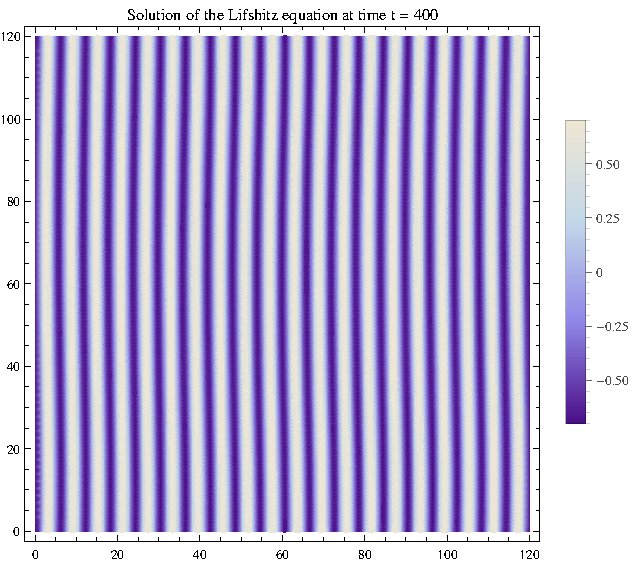
\includegraphics[width=.9\linewidth]{img/chap1/sol_Lif_t400.png}
	\caption{}
	\label{lif_t400}
\end{subfigure}
\caption{Time evolution of a field obeying the equation of movement derived from the (time dependent) Lifshitz action. We see that the structure evolves toward a modulated steady state.}
\label{fig:evol_strip}
\end{figure}


\begin{figure}[htp]
\begin{center}
\includegraphics[scale=1]{img/chap1/phase_diagram_2.pdf}
\caption{Typical phase diagram of a system described by the Lifshitz model. The Lifshitz point is labelled $L$. Temperature varies along the vertical axis while the horizontal axis accounts for the variation of an extra parameter $\rho_0$.}
\label{fig:phase_diagram}
\end{center}
\end{figure}

A crucial feature of this phase diagram is the intersection point of the modulated, ferromagnetic and antiferromagnetic phases, called the Lifshitz point ($L$ in fig. \eqref{fig:phase_diagram}). 
Historically, the manganese phosphite (MnP) magnetic crystal was one of the first systems in which a Lifshitz point could be detected. Moreover, the entire phase diagram around the Lifshitz point of the MnP crystal could be inferred with high precision from experimental measurements \cite{MnP}.
The phase diagram of a Lifshitz system is bidimensional: one axis being the temperature, and the other and extra parameter -- called $\rho_0$ from now on, whose precise meaning depends on the physical nature of the studied system.
In the case of the MnP magnetic crystal, the tunable $\rho_0$ parameter is an external magnetic field applied to the crystal, while the order parameter  is the local magnetization of the atoms. In the modulated phase, it is the angle between the direction of the local magnetization and a direction of reference that is spatially modulated.

Experiments also provide evidence of Lifshitz point existence in ferroelectrics and liquid crystals.

\subsubsection{The Lifshitz model}

The Lifshitz model is a field theory, describing a vector field $\phi$ whose components will be denoted $\phi_i$.
If we like to think in terms of magnetic systems, like the MnP cristal, we can say that $\phi(x)$ is the coarse-grained magnetization at position $x$.
 To write the action for the Lifshitz model, we choose a basis $(\mathbf{e_n})_{1 \leq n \leq d}$. We decide that this basis is such that its first $m$ vectors span the $m$ dimensional $\sslash$ subspace, while of course the remaining $d-m$ base vector span the $\perp$ subspace. In this basis, the Lifshitz action is
\begin{equation}
S = \int_x \sum_{i=1}^N \left( \frac{1}{2} \left(\sum_{n_\perp=m+1}^{d}\frac{\partial \phi_i}{\partial x_{n_\perp}} \mathbf{e_{n_\perp}}\right)^2 + \frac{\rho_0}{2} \left(\sum_{n_\sslash=1}^{m}\frac{\partial \phi_i}{\partial x_{n_\sslash}} \mathbf{e_{n_\sslash}}\right)^2 + \frac{\sigma_0}{2} \left(\sum_{n_\sslash=1}^{m} \frac{\partial^2 \phi_i}{\partial x_{n_\sslash}^2} \mathbf{e_{n_\sslash}}\right)^2 \right) + U(\phi)
\end{equation}
As we want to model the broadest possible class of physical systems, we will say that $U$ is an almost completely arbitrary potential. We only ask for it to have the $O(n)$ symmetry, \textit{i.e.} to be a function of $\rho \define \phi_i \phi_i/2$.

From now on we will use the self-explanatory shorthand notation
\begin{equation}
H[\phi] = \int_x \left( \frac{1}{2}(\p{\perp} \phi)^2 + \frac{\rho_0}{2}(\p{\sslash} \phi)^2 + \frac{\sigma_0}{2} (\p{\sslash}^2 \phi)^2 + U(\rho) \right)
\end{equation}

We see that this action closely resemble the well known action of the $O(n)$ model
\begin{equation}
S_{O(N)} = \int_x \left( \frac{1}{2}(\partial \phi)^2 + U(\rho) \right)
\end{equation}
Namely, we recover it if we set $\rho_0 = 1$ and $\sigma_0 = 0$. We see that what differentiates the Lifshitz and $O(n)$ action is on one hand the presence a non trivial (\textit{i.e.} different from 1) $\rho_0$, breaking the $O(d)$ invariance, and on the other hand the presence of an extra term involving a Laplacian squared. Clearly, these two modifications must be responsible for the appearance of spatially modulated structures, but why exactly? 
We can gain a useful intuition of why a spatially modulated structure is closely linked to the existence of a Laplacian squared term in the action by looking at a microscopic version of our model. 

\subsection{A discrete counterpart: the anisotropic Ising model}

Stricto sensu the discrete counterpart of the Lifshitz model would be an anisotropic Heisenberg model, but to simplify things - without changing the essence of the argumentation - we consider an anisotropic Ising model instead.

First, let us consider a chain of Ising spins with the Hamiltonian
\begin{equation}
H_{\text{chain}} \define - J \sum_i S_i S_{i+1}
\end{equation}
We know that if $J$ is positive, the interaction is ferromagnetic, whereas is $J$ is negative, the interaction is antiferromagnetic. 
The antiferromagnetic order already shows some kind of spatial modulation, but it only exists at zero temperature! 
The idea to make a spatially modulated order survive at non zero temperatures is to consider a second neighbors \textit{antiferromagnetic} interaction, together with a first neighbors \textit{ferromagnetic} interaction:
\begin{equation}
H_{\text{chain}} = - J_1 \sum_i S_i S_{i+1} - J_2 \sum_i S_i S_{i+2}
\end{equation}
However, for a long range order to exist at finite temperature, we need to work in two dimensions or more, \textit{i.e.} to trade our spin chain for a spin lattice:
 \begin{equation}
 H_{\text{lattice}} \define - \sum_i \left( J_0 \sum_{\delta_\perp} S_i S_{i+\delta_\perp} + J_1 \sum_{\delta_\sslash} S_i S_{i+\delta_\sslash} + J_2 \sum_{\delta_\sslash} S_i S_{i+2 \delta_\sslash} \right)
 \end{equation}
 Qualitatively, the competition between ferromagnetic and antiferromagnetic interactions will produce a spatial modulation of the spins at non zero temperatures, at least for some values of the interaction strengths ratio $J_2/J_1$. 
 The existence of a stripped phase indeed is a well known feature of this model \cite{ANNNI}, called the ANNNI (axial next-nearest neighbour Ising) model.
 
 Now, what is the link between this discrete spin lattice Hamiltonian, and our continuous action?
Note that a sum on nearest neighbors can be rewriten in terms of a discrete Laplacian on the lattice, while a sum on next-nearest neighbors involves a discrete Laplacian squared:
\begin{equation}
H_{\text{lattice}} = -\sum_i \left( \kappa S_i^2 + J_0 S_i \Delta_\perp S_i + (J_1 + 4 J_2) S_i \Delta_\sslash S_i - J_2 S_i \Delta_\sslash^2 S_i \right)
\end{equation}
where we introduced the differential operators on the lattice:
\begin{align}
\Delta_\sslash S_i = \sum_{\delta_\sslash} S_{i-\delta_\sslash} - 2 S_i + S_{i+\delta_\sslash} \\
\Delta_\perp S_i = \sum_{\delta_\perp} S_{i-\delta_\perp} - 2 S_i + S_{i+\delta_\perp} \\
\Delta_\sslash^2 S_i = \sum_{\delta_\sslash} -S_{i-2\delta_\sslash} +  4 S_{i-\delta_\sslash} - 4 S_i + 4S_{i+\delta_\sslash} - S_{i+2\delta_\sslash}
\end{align}
This rewriting in terms of discrete differential operators makes it clear that this Hamiltonian is the discrete --microscopic-- counterpart of the Lifshitz action. We now understand --at least intuitively-- the origin of the spatially periodic structures (shown in fig. \eqref{fig:evol_strip}) the field of the Lifshitz model exhibits. They exist because of the competition between \textit{nearest neighbors ferromagnetic interactions} (giving rise to the $\Delta_\sslash$ term in the Lifshitz action), and \textit{next-nearest neighbors antiferromagnetic interactions} (giving rise to the $\Delta_\sslash^2$ term in the Lifshitz action).

At this point a question arises: why work with a Lifshitz coarse-grained field theory, since we have a better physical understanding of an underlying microscopic model? What is more, in passing to a continuous theory, we lose information about the microscopic underlying lattice. 
This is actually not a problem since the statistical quantities we are interested in computing -namely the critical exponents of the phase transition- are universal; they do not depend on the specific microscopic model, if the symmetries of this model were carefully implemented in the continuum limit. Actually, passing to a field theory is even advantageous as it frees us of the irrelevant microscopic details. 
Even more crucial is the fact that field theories are the objects of choice for application of the powerful methods of the renormalization group, which we will now describe.
\Chapter{The renormalization procedure}{Introduction to the nonperturbative renormalization techniques}

At the so-called Lifshitz critical point, three phases intersect. This is rather unsual, so we expect the physics of the vicinity of this point to be of special interest. To investigate it, we would like to compute the critical exponents associated to this transition point. To this end, we used the powerful machinery of the renormalization group, and more precisely of one particular implementation of the renormalization ideas: the nonpertubative renormalization group.

In this chapter we propose first a very general introduction to the ideas and concepts of the renormalization. Then we focus on the nonperturbative renormalization group techniques.

\section{Introduction to the renormalization group}

\section{The nonperturbative renormalization group}

\chapter{The Lifshitz critical point: methods and results}

As we have seen, the Wetterich equation governs the flow of the scale-dependent effective action $\Gamma_t$. Solving directly this differential equation to find $\Gamma_t$, though in theory possible, is in practice very difficult. Indeed the $\Gamma_t$ depends on the (background) field $\phi$, a function of the momentum. Determining completely $\Gamma_t$ requires knowing its value for all functions $\phi$. 

So, instead of solving directly the Wetterich equation, we start from a reasonable functional form for $\Gamma_t$ with unknown coefficients, we plug it in the Wetterich equation to get flow equations for this coefficients, and we solve these equations.

If we assume that it is analytic in the potential, the effective action can be written as the infinite sum
\begin{equation}
\Gamma_t[\phi] = \int_{x} \left( m_0 (\partial \phi(x))^2 + m_1 (\partial \phi(x)^2)^2 + ... + n_0 (\partial^2 \phi(x))^2 + ... + l_0 \phi(x)^2 + l_1 \phi(x)^3 +... \right)
\end{equation}

This expression can be further simplified if the system under study has some invariance properties. The simplest model having such an invariance is the Ising one, whose microscopic Hamiltonian is invariant under the action of the $\mathds{Z}_2$ symmetry group. If we chose a regulator that preserves this symmetry, it is clear that the effective action $\Gamma_t$ must also be invariant under $\mathds{Z}_2$. The most general expression for $\Gamma_t$ that preserves this symmetry is
\begin{equation}
\label{eq:ising_anzatz}
\Gamma_t^{\text{Ising}}[\phi] = \int_{x} \sum_{i,j \in \mathds{N}} Z_{t,ij} (\partial \phi(x))^{2i} \phi(x)^{2 j}
\end{equation}
The strategy is now simple:
\begin{itemize}
\item Compute $\Gamma_t^{(2)}(x,y)$ from \eqref{eq:ising_anzatz}
\item Plug the result in the right hand side of the Wetterich equation
\item Deduce the flow equation for $Z_{t,ij}$: $\p{t} Z_{t,ij} = F_{i,j}\left( {Z_{t,kl}} \right)$
\end{itemize}
Following this procedure we went from a functional differential equation to a set of simple differential equations. Solving this set of flow equations gives us a complete knowledge of the model. In particular solving the fixed point equations $0 = F_{i,j}\left( {Z^*_{kl}} \right)$ will give us access to the critical properties of the Ising model: critical exponents, critical potential,... Note that for the moment no approximations have been made!

In practice however we know that the lowest degree terms in $\partial \phi$ and $\phi$ will have the most significant contribution to the flow. Therefore we can make the approximation of cutting the development at some order. This has the great practical advantage of reducing the number of flow equations to solve to a finite number. Note that other approximation schemes are possible (development in powers of the field, BMW scheme...). We will not talk about these.

\section{An Anzatz for the Lifshitz scale-dependant effective action}
We recall that the Lifshitz microscopic Hamiltonian is

\begin{equation}
H[\phi] = \int_x \left( \frac{1}{2}(\p{\perp} \phi)^2 + \frac{\rho_0}{2}(\p{\sslash} \phi)^2 + \frac{\sigma_0}{2} (\p{\sslash}^2 \phi)^2 + U(\rho) \right)
\end{equation}
where $\rho = \phi_i \phi_i/2$. 
The Lifshitz Hamiltonian has the $O(n)$ symmetry\footnote{Meaning that a rotation of the $n$-dimensional field $\phi$ leaves the Hamiltonian invariant: $H[\mathcal{R}(n)\phi] = H[\phi]$ if $\mathcal{R}$ is an orthogonal $n \times n$ matrix.}, therefore the scale-dependent effective action should also have this symmetry. Moreover the kinetic term in the Lifshitz Hamiltonian decomposes into two parts:
\begin{itemize}
\item $\int_{x} \frac{\rho_0}{2}(\p{\sslash} \phi)^2 + \frac{\sigma_0}{2} (\p{\sslash}^2 \phi)^2$, invariant under $\left(x_\sslash,x_\perp \right) \rightarrow \left(\mathcal{R}(m) x_\sslash, x_\perp\right)$
\item $\int_{x} \frac{1}{2}(\p{\perp} \phi)^2$, invariant under $\left(x_\sslash,x_\perp \right) \rightarrow \left(x_\sslash, \mathcal{R}(d-m) x_\perp\right)$
\end{itemize}
Since the scale-dependent effective action must satisfy these symmetry properties, its most general form is
\begin{equation}
\Gamma_k[\phi] = \int_{x} U(\rho) + \left( \frac{1}{2} Z_\perp(\rho) (\partial_\perp \phi)^2 + \frac{1}{4} Y_\perp(\rho) (\partial_\perp \rho)^2 + ... \right) + \left( \frac{1}{2} \rho_0(\rho) (\partial_\sslash \phi)^2 + ... \right) + \left( \frac{1}{2} Z_\sslash(\rho) (\partial_\sslash^2 \phi)^2 + ... \right)
\end{equation}

It turns out to be a very good approximation to cut the derivative expansion to first order \footnote{To compute critical exponents, one does not need to take into account the full momentum dependence of the theory. However for computing correlation function the momentum dependence is essential. Were we to compute these quantities, we will probably have to go further in the derivative expansion}. That is to say, we make the approximation
\begin{eqnarray}
\frac{1}{2} Z_\perp(\rho) (\partial_\perp \phi)^2 + \frac{1}{4} Y_\perp(\rho) (\partial_\perp \rho)^2 + ...  \simeq  \frac{1}{2} Z_\perp(\rho) (\partial_\perp \phi)^2  \\
 \frac{1}{2} \rho_0(\rho) (\partial_\sslash \phi)^2 + ...  \simeq  \frac{1}{2} \rho_0(\rho) (\partial_\sslash \phi)^2 \\
\frac{1}{2} Z_\sslash(\rho) \partial_\sslash^2 \phi)^2 + ... \simeq \frac{1}{2} Z_\sslash(\rho) \partial_\sslash^2 \phi)^2
\end{eqnarray}
Moreover, we make the approximation that the field renormalizations $Z_\perp(\rho)$, $\rho_0(\rho)$ and $Z_\sslash(\rho)$ do not depend on the field. So, the definitive form of the Anzatz we chose for $\Gamma_t$ is
\begin{equation}
\label{eq:gamlif}
\Gamma_t[\phi_i] = \int_x \left ( \frac{Z_\perp}{2} (\partial_\perp \phi)^2 + \frac{\rho_0}{2} (\partial_\sslash \phi)^2 + \frac{Z_\sslash}{2} (\partial_\sslash^2 \phi)^2 + U(\rho) \right )
\end{equation}
This is the form of the Lifshitz scale-dependent effective action we have worked on during this internship.
Though this does not appear explicitly, the field renormalizations and the effective potential $U$ depend on the renormalization time $t$. As we are going to see, the $t$ dependence of $Z_\perp$ and $Z_\sslash$ gives rise to non trivial anomalous dimensions. The anomalous dimensions are expected to act as a small correction to the value of the critical exponents. At first order, we can thus assume trivial anomalous dimensions. This amounts to forgetting the $t$ dependence of $Z_\sslash$ and $Z_\perp$ in the effective action. This approximation is called the \textit{local potential approximation}.


 We will now make use of the Wetterich equation to know how this quantities change through the renormalization process. Then we will use this knowledge to derive the critical exponents.

\section{The Lifshitz renormalization flows}

\subsection{Dimension-driven versus fluctuations-driven flows}
We recall that looking at the mean field version of a theory consists in neglecting all fluctuations of the field. Therefore, in the case of a mean field theory, the renormalization procedure -- average on fluctuations up to a certain scale, definition of an effective Hamiltonian and rescaling -- only requires rescaling. 
The conclusion is that the renormalization flows of mean field theories' coupling constants are only due to their dimension.

If we wish to go beyond the mean field approximation, we have to take into account the fluctuations of the field.
They are often small compared to the mean value of the field, meaning that their contribution to the flows will be small compared to the contribution coming from the mean field theory. In other words, the fluctuation-driven part of a renormalization flow is generally small compared to its dimension-driven part. 
Wishing to concentrate on the small non-trivial part of the flow: the fluctuation-driven part, we define \textit{dimensionless coupling constants}, that are by construction subject to a fluctuation-driven flow only.\footnote{Numerically, if we want to track the contribution to the flow of fluctuations $10^{12}$ weaker than the mean field contribution, we must achieve at least $12$ digits precision, which is often rendered impossible by rounding errors. In this context using dimensionless coupling constant indeed seems an excellent idea!}

With these ideas in mind, we define the following dimensionless quantities 


\begin{center}
\begin{tabular}{|c|c|c|}
\hline
$q_\sslash^2 = k^{2 \theta} y_\sslash$ & $q_\perp^2 = Z_\sslash Z_\perp^{-1} k^{4\theta} y_\perp$ & $\rho_0 = Z_\sslash k^{2\theta} \bar \rho_0$\\ 
\hline 
$R(q_\perp^2,q_\sslash^2) = Z_\sslash k^{4\theta} y_\sslash^2 r(y_\perp, y_\sslash)$ & $U(\rho) = Z_\sslash k^{d_m} u(\bar{\rho})$ & $\rho = Z_\sslash^{-1} k^{-4\theta + d_m} \bar{\rho}$ \\ 
\hline 
\end{tabular}
\end{center}

Note that given the relation
\begin{equation}
\theta = \frac{2-\eta_\perp}{4-\eta_\sslash}
\end{equation}
we have a certain liberty relative to the adimensionning of the physical quantities. For example we can define $\rho_0 = Z_\sslash k^{2\theta} \bar{\rho_0}$ or $\rho_0 = Z_\perp^{1/2}Z_\sslash^{1/2}k\bar{\rho_0}$. These two definitions lead to two different $\bar{\rho_0}$ functions, but the two functions have \textit{the same dimensional flow}.. Here we chose the adimensionning such that $Z_\sslash$ simplifies everywhere in the propagators. 

\subsection{Flow of the potential}
From the shape of the potential, we can tell in which phase we are. Therefore knowing how the potential changes with $t$ is of paramount importance. We shall thus start with the derivation of the flow equation for the potential.

We see that 
\begin{equation}
U(\rho_0) = \delta(0)^{-1} \Gamma_t[ \phi] |_{\phi(x) = \phi_0}
\end{equation}
where $\phi_0$ is some uniform (in direct space) configuration of the field, and where $\rho_0 = \phi_{0i} \phi_{0i}/2$. Note that if we were to work on a finite-size system, the $\delta(0)^{-1}$ term would be replaced by the volume of the system. Therefore it plays the role of the system volume for the infinite size system we consider here.

We take a derivative with respect to $t$ to get an expression for the flow of the potential, and we plug in the Wetterich equation on the right hand side:
\begin{equation}
 \partial_t U(\rho_0) = \delta(0)^{-1} \partial_t \Gamma = \frac{1}{2 \delta(0)} \hat \partial_t \tr{\log\left( \Gamma_t^{(2)} + R_t  \right)}
\end{equation}
This is the flow equation for the potential!\footnote{It should be noted that we only derived the flow equation of the potential for a constant field configuration. This is of no importance as we do not need the \textit{functional} dependence of the potential, $(x \mapsto \rho(x)) \mapsto U(\rho(x))$ but only its ``digital'' dependence $\rho_0 \mapsto U(\rho_0)$ to characterize it completely.}

From eq. \eqref{eq:gamlif} we compute the second derivative of the effective action in Fourier space:
\begin{equation}
\Gamma^{(2)}_{ij}(p,q) = 
\left( \delta_{ij} \left(Z_\perp p_{\perp}^2 +\rho_0 p_{\sslash}^2 +Z_\sslash (p_\sslash^2)^2 + U'(\rho (x))\right)+\phi_i(p) \phi_j(q) U''(\rho (x)) \right) \delta(p+q)
\end{equation}
We can decompose the $\Gamma^{(2)}_{ij}$ function on a orthogonal the projector on the direction of the field $\Pi^a_{i,j} \define \delta_{ij} - \frac{\phi_i \phi_j}{2 \rho}$ and on the projector orthogonal to it $\Pi^r_{i,j} = \frac{\phi_i \phi_j}{2 \rho}$.
This allows us to easily rewrite the regularized full propagator appearing in the Wetterich equation:
\begin{equation}
\label{eq:gam2}
\left( \Gamma^{(2)}_{ij}(p,q) + R_t(p,q) \right)^{-1} = \left( G_a(q) \Pi^a_{ij} + G_r(q) \Pi^r_{ij} \right) \delta(p+q)
\end{equation}
where we used the radial and angular propagators:
\begin{align}
G_r(q) \define \frac{1}{Z_\sslash q_\sslash^4 + Z_\perp q_\perp^2 + \rho_0 q_\sslash^2 + R_t(q)  + U'(\rho) + 2 \rho U^{(2)}(\rho)} \\
G_a(q) \define \frac{1}{Z_\sslash q_\sslash^4 + Z_\perp q_\perp^2 + \rho_0 q_\sslash^2 + R_t(q) + U'(\rho)}
\end{align}
We can now rewrite in a more explicit way the Wetterich equation:
\begin{equation}
\p{t} \Gamma_t = \frac{1}{2} \int_q \left(  G_a(q) \Pi^a_{ij} + G_r(p) \Pi^r_{ij} \right) \p{t} R_{t,ij}(q)  = \frac{1}{2} \int_q \left(  G_a(q) + (n-1)G_r(p) \right) \p{t} R_{t}(q) 
\end{equation}
Note that the radial (massive) propagator appears once whereas the angular (massless) propagator appears $n-1$ times in the flow equation. This is of course because as soon as we choose a direction for the field $\phi$, the  $O(n)$ invariance is no longer explicit (though the equation is of course still $O(n)$ invariant). Therefore, a massive Goldstone mode and $n-1$ massless modes appear, in accordance with Goldstone's theorem.

Imposing now that the field is constant, we have for the flow of the potential
\begin{equation}
\p{t} U(\phi_0) = \frac{1}{2} \int_q \left( G_r(q)\atpt{unif} + (n-1)G_a(q)\atpt{unif} \right) \p{t} R_t(q)
\end{equation}
This is as far as we can get without giving explicitly a form to the regulator. 
At this point, it is a customary procedure to introduce standard functions called \textit{threshold functions} in order to lighten the notations. Their definition can be found in appendix \eqref{app:thresholds}.

Passing to dimensionless quantities the flow of the potential can be expressed in terms of the $l$ threshold function:
\begin{equation}
\label{eq:flow_u}
d_t u_t(\rho) = -d_m u_t(\rho) +(\theta \eta_\sslash + d_m - 4 \theta) \rho u_t'(\rho) + 8 v_m v_{d-m} \left( l_0^{dm}\left(u_t'(\rho) + 2 \rho u_t''(\rho) \right) + (n-1)l_0^{dm}\left(u_t'(\rho)\right) \right)
\end{equation}
This is a second order, nonlinear differential equation, that can be solved at least numerically, once we have chosen an explicit form for the regulator (in order to compute the $l_0$ threshold function), and once we know the values of $\rho_0$, $\eta_\sslash$ and $\theta = (4-\eta_\sslash)/(2-\eta_\perp)$. As we are going to see now, the values of $\eta_\sslash$ and $\eta_\perp$ are related to the flows of $Z_\sslash$ and $Z_\perp$.

\subsection{Flow of the field renormalizations.}

What we call field renormalizations are the prefactors $Z_\sslash$ and $Z_\perp$. We will briefly explain why $\p{t} \log Z_\perp \sim - \eta_\perp$. The argument is of course exactly the same for $\eta_\sslash$. 

\subsection{The anomalous dimension in the orthogonal direction.}

\subsubsection{Flow of the field renormalization and anomalous dimension}

From the inverse full propagator (given by eq. \eqref{eq:gam2}) we can retrieve the field renormalization in the $\perp$ direction:
\begin{equation}
\label{eq:etaperp}
\frac{d}{dp_\perp^2} \Gamma^{(2)}_{ij}(p,q) = \delta_{ij} \delta(p+q) Z_\perp
\end{equation}
and because $\gam^{(2)}$ flows accordingly to the Wetterich equation, from the above equation we can compute the flow of $Z_\perp$. 
Note that this flow will depend on the external impulsion $p$. From dimensional analysis it is easy to see that
\begin{equation}
 Z_\perp \xrightarrow[p \rightarrow 0,\text{~} k>0]{} C k^{-\eta_\perp}
 \end{equation} 
 where $C$ is a dimensionless constant factor. So, at vanishing $p$, the flow of $Z_\perp$ is linked to the anomalous dimension:
 \begin{equation}
 - \p{t} \log Z_\perp \xrightarrow[p \rightarrow 0,\text{~} k>0]{} \eta_\perp
 \end{equation}
 We shall use this relation to compute the anomalous dimension from the flow of $Z_\perp$.
 To express $\eta_\perp$ we can simply take the limit of vanishing external moment of equation $\eqref{eq:etaperp}$. This gives
\begin{equation}
\eta_\perp = -\frac{1}{\delta(0) Z_\perp} \hat{\p{t}} \lim_{p \rightarrow 0} \frac{d}{dp_\perp^2} \left( \Gamma^{(2)}_{ii}(p,-p) \atpt{unif} \right)
\end{equation}
The index $i$ is still not fixed. To set things, we decide that $1$ is the direction of the uniform field $\phi_0$. Then we can either chose $i=1$, or $i \neq 1$ (all directions orthogonal to the field are equivalent). We made here the choice $i \neq 1$, because we know that in that case the expression we obtain for $\eta_\perp$ is exact in the $n \rightarrow \infty$ limit. Explicitly, we chose $i=2$.
Now all we need to do to obtain the explicit expression of $\eta_\perp$ in terms of the propagators is compute $\p{t} \Gamma^{(2)}_{22}(p,-p) \atpt{unif}$, derive it with respect to $p_\perp$ and take the limit of vanishing $p$. As the computation is rather lengthy, we will only give the important intermediate steps.

\subsubsection{Computation of the flow}
\label{sec:etaperp}
Notice that we can intertwine $\p{t}$ and $\atpt{unif}$ since the uniform field does not flow. 
Therefore all we have to compute is the second functional derivative of the effective action's flow $ \left(\p{t} \Gamma\right)^{(2)}_{22} \atpt{unif}$. This double functional derivative gives rise to two terms, one involving a 4-points function $\gam^{(4)}$ and one involving two 3-points functions $\gam^{(3)}$.


All the dependence on the external momentum $p$ of the first term is held by the 4-points function. Here, because the kinetic terms in the effective action only involve two fields, every $n$-points function for $n \geq 3$ is momentum independent. Therefore this first term does not contribute to the anomalous dimensions.
So we keep only the second term, whose contribution to $\p{t} \left ( \Gamma^{(2)}_{2,2}(q,-q) \atpt{unif} \right )$  we call $D(p)$. Dropping for simplicity the discrete indices, that are summed upon in the trace, we have
\begin{equation}
D(p) = \frac{-1}{2} \hat{\p{t}} \int_q \tr{ G(q)\Gamma^{(3)}_{2}(q, q + p) G_{}(q + p) \Gamma^{(3)}_{2}(q + p, q) }
\end{equation}
where $G_{ij}(p,q) = \left ( \Gamma^{(2)}(p,q) + R_t(p)\delta(p+q) \right )^{-1}_{ij}$ is the full propagator.

Computing explicitly the $\gam^{(3)}_{i2j}$ function, which, like the 4-points function, does not depend on the external momentum, we can rewrite the anomalous dimension in a compact way:
\begin{align}
\eta_\perp = \frac{1}{Z_\perp} \tr{\Pi^r\Gamma^{(3)}_{2} \Pi^a \Gamma^{(3)}_{2}} \hat{\p{t}} \lim_{p \rightarrow 0} \frac{d}{dp^2_\perp} \int_q G_r(q) G_a(p+q)
\end{align}
This is a very general expression, holding as soon as the effective action has no kinetic terms of order $\geq 3$ in the field. In particular, it also holds for the $O(n)$ model.
More specifically here we have $\tr{\Pi^r\Gamma^{(3)}_{2} \Pi^a \Gamma^{(3)}_{2}} = 2 \rho \left ( U^{(2)}(\rho) \right )^2$

\subsubsection{Action of the derivative with respect to the momentum}
Computing the derivative is a lengthy, error-prone computation. We used Mathematica to do it. The procedure is given in appendix \ref{app:mathematica}.
We finally obtained for $\eta_\perp$ the following expression, using an $m$ threshold function defined in appendix \ref{app:thresholds}.
\begin{equation}
\label{eq:flow_perp}
\eta_\perp = 64 \frac{v_m v_{d-m}}{d-m} \rho \left( u^{(2)}(\rho) \right)^2 m_{0,2220}
\end{equation}

\subsection{The anomalous dimension in the parallel direction, and the flow of $\rho_0$.}

The two other computations are very similar. In particular the flow of $\rho_0$ should be given by the flow of $Z_\perp$ with the role of the $\perp$ and $\sslash$ directions exchanged, because of the symmetry between $\rho_0$ and $Z_\perp$. The formula for $\eta_\sslash$ is more complicated as it involves fourth powers of the momentum.
\begin{align}
\label{eq:flow_rho}
d_t \rho_0 = -\theta \left(2-\eta_\sslash\right) \rho_0 - 64 \frac{ v_{d-m} v_m}{m} \rho \left( u^{(2)}(\rho) \right)^2 m_{1,2202} \\
\eta_\sslash = 32 v_{d-m} v_m \rho \left( u^{(2)}(\rho) \right)^2 
\label{eq:flow_ss}
\Bigg[ m_{1,3100} - \frac{1}{2} k_{1,2100} + \frac{1}{m}\left( -12 s_{1,4102} + 12v_{1,31002} -2w_{1,2102} \right) \\
{}+ \frac{1}{m(m+2)}\left( 48 t_{1,5104} -72 z_{1,4104} +12 u_{1,3104} +16 y_{1,3104} -2 x_{1,2104} \right) \Bigg]
\end{align}
Where $s$, $t$, $s$, ... are again threshold functions.


Equations \eqref{eq:flow_u}, \eqref{eq:flow_perp}, \eqref{eq:flow_rho}, \eqref{eq:flow_ss} tell us how the potential, $\rho_0$ and the anomalous dimensions are modified under the action of the renormalization group. With these equations, we can now compute the critical exponents of the Lifshitz point. 



\subsection{Solving the fixed point equations}

To compute the critical exponents at the Lifshitz point now that we have derived the flow equations of the couplings, several approaches are possible. 
They all rely on the flow equation for the potential,
\begin{equation}
d_t u_t(\rho) = -d_m u_t(\rho) +(\theta \eta_\sslash + d_m - 4 \theta) \rho u'_t(\rho) + 8 v_m v_{d-m} \left( l_0^{dm}\left(u'_t(\rho) + 2 \rho u''_t(\rho) \right) + (n-1)l_0^{dm}\left(u'_t(\rho)\right) \right)
\end{equation}
This equation is perhaps the most important of the four flow equations we have derived. Indeed the shape of the potential tells us were we are in the phase diagram (fig. \eqref{fig:phase_diagram}). 

\begin{figure}[htp]
\begin{center}
\includegraphics[scale=0.6]{img/chap4/u_flow_ising.pdf}
\caption{The potential for the Ising model at different times (local potential approximation was used). The accumulation of shapes tells us that we started close from a fixed point.}
\label{fig:u_flow_ising}
\end{center}
\end{figure}

An idea is to start from a shape for the potential at the microscopic scale, and plug it as an initial condition of the flow equation to see how the potential evolve in time. Here we took $u_{t=0}(\rho) = u_0 + \sigma \rho + u_4 \rho^2$ for the initial condition. We see that $\sigma$ is the temperature at the microscopic scale.
If at first the potential is almost stationary, that means we have started close from a critical point.
 By trial and error, \textit{i.e.} by fine-tuning of the temperature at microscopic scale, we can start closer and closer from the critical point. Once we have a sufficient precision, we can compute the critical exponents associated to this critical point. We tried this method with some success on the Ising model (fig. \eqref{fig:u_flow_ising}).
 
Several drawbacks entail this method. First, we have to solve a partial differential equation, which take some time. Secondly and more importantly, once we have found a critical point, it is hard to know which one it is if there exist several ones (which is the case for the Lifshitz model in $d = 3$).

For all this reasons, we used another approach: solving directly the fixed point equation, which is only a differential equation. This approach has, as we are going to see, the extra advantage of letting one locate with ease a fixed point of interest.

The equation we are interested in solving is 
\begin{equation}
0 = -d_m u(\rho) +(\theta \eta_\sslash + d_m - 4 \theta) \rho u'(\rho) + 8 v_m v_{d-m} \left( l_0^{dm}\left(u'(\rho) + 2 \rho u''(\rho) \right) + (n-1)l_0^{dm}\left(u'(\rho)\right) \right)
\end{equation}
Recalling that the $l_0$ functions are defined by an integral, we see that this is an implicit second order nonlinear differential equation, whose general solution is not known. One may wonder if there exists a clever choice of regulator that let us compute the integral, thus turning the nonlinear differential algebraic equation into a simple nonlinear differential equation. 
For the Ising model (in the local potential approximation), such a form of regulator is indeed known\footnote{It is the so-called $\theta$ regulator, $R_t(q)= (k^2-q^2) \theta\left(1-q^2/k^2\right)$}. For the Lifshitz model, it is not known if there exists a regulator allowing one to compute the integral explicitly. However we found a form of regulator allowing one to compute the integral approximately. Under this approximation -- which is explained and justified in appendix \ref{app:approx} -- the fixed point equation becomes
\begin{equation}
\label{eq:u_approx}
0 = u(\rho) - a(\theta, \eta)  \rho u'(\rho) + b_1(\theta, \eta) b_2(\theta, \eta, \rho_0) \left( \frac{1}{1 + \rho_0 + u'(\rho) + 2 \rho u''(\rho)} + \frac{n-1}{1+\rho_0+u'(\rho)} \right)
\end{equation}
This is an explicit second order nonlinear differential equation that depends on three parameters: $\eta$, $\theta$ and $\rho_0$. 
Of course the temperature also is a tunable parameter, appearing in the initial condition of the equation. Indeed, we have $u'(\rho=0) = \sigma$, the temperature. $u(0)$ is also linked to the temperature by $u(0) = n b_1 b_2/(1+\sigma)$.

By simply setting the value of the couple $(\sigma, \rho_0)$ we can place ourselves at any point of the two-dimensional phase diagram of the Lifshitz model.
Since this is the \textit{fixed point equation} for the potential, solving it returns the potential at the critical point $(\sigma, \rho_0)$. What happens when $(\sigma, \rho_0)$ is not a critical point? It turns out that the then unphysical solution of the fixed point equation blows up at some finite value of the field $\rho_{\text{sing}}(\sigma, \rho_0)$. 

This provides us with an easy way of finding fixed points. They correspond to points where the potential is defined for all values of the field, \textit{i.e.} to points such that $\rho_{\text{sing}}(\sigma, \rho_0)$ diverges. See fig. \eqref{fig:on_fp} for an illustration of this procedure in the simpler $O(n)$ case, which we tried before the Lifshitz case. 

\begin{figure}[htp]
\centering
\begin{subfigure}{.55\textwidth}
	\centering
	\includegraphics[width=.9\linewidth]{img/chap4/on_d3_n3.pdf}
	\caption{$d=3$}
	\label{on_d_3}
	\end{subfigure}%
\begin{subfigure}{.55\textwidth}
	\centering
	\includegraphics[width=.9\linewidth]{img/chap4/on_d2p6_n3.pdf}
	\caption{$d=2.6$}
	\label{on_d_2p6}
\end{subfigure}
\caption{Plot of the (numerically computed) explosion location $\rho_{\text{sing}}$ for the $O(n)$ model in the local potential approximation. We see that in $d=3$ only two physical solutions exist. They are the Gaussian fixed point, at $\sigma = 0$, and the Wilson-Fisher fixed point at its left. A second non trivial fixed point appears at $d = 8/3 \simeq 2.6$.}
\label{fig:on_fp}
\end{figure}

Once the critical temperature and $\rho_0$ are found, knowing the potential solution of the fixed point equation at this critical point we can compute the critical exponents. This method has already been applied successfully to the Ising \cite{CodelloIsing} and $O(n)$ \cite{CodelloOn} models. This was the first time it was tried on the Lifshitz model.
 The Lifshitz case is a slightly more complicated as it has two dimensional phase space, instead of a one dimensional one. This means that we must solve a system of two equations: the fixed point equation on the potential, and the fixed point equation on $\rho_0$, in order to fix the value of the two parameters.

We have not yet discussed the fate of the free parameters $\theta$, $\eta_\sslash$. In the local potential approximation, which we have considered here, they take their mean field value: $\theta \simeq \theta_{\text{mean field}} =  1/2$, $\eta_\sslash \simeq \eta_{\sslash\text{~mean field}} = 0$.
Beyond the mean field approximation, we must make use of the equations \eqref{eq:flow_perp}, \eqref{eq:flow_ss} to constrain the anomalous dimensions. We have derived these two equations, but had no time to go beyond mean field and use them.


To sum up, we have adopted the following strategy:
\begin{itemize}
\item Start at $d=d_c^>$, where mean field is exact in the sense that $\rho_0 = 0$.
\item Slightly decrease the dimension: $d \rightarrow d - \delta d$. 
\item Find the temperature of the Lifshitz point, by fine tuning of $\sigma$, using the fixed point equation on $u$ (eq. \eqref{eq:u_approx}).
\item Find how the value of $\rho_0$ has been modified by this shift in dimension and in temperature, using the fixed point equation on $\rho_0$ (eq. \eqref{eq:flow_rho}).
\item Go back to step two.
\end{itemize}
We have followed this algorithm until we reached $d=3$, at which point our results concerning critical exponents could be compared with the ones obtained by other means.

\subsection{Fixed point potential at the Lifshitz critical point}

\begin{figure}[htp]
\begin{center}
\includegraphics[scale=1]{img/chap4/emergence_lif.pdf}
\caption{Emergence of the Lifshitz fixed point (at the left of the $\sigma = 0$ Gaussian fixed point), when $d$ is slightly lowered, starting from $d_c^>$. Here we have chosen $m=1$ (and thus $d_c^> = 4.5$) and $n=3$.}
\label{fig:emergence_lif}
\end{center}
\end{figure}

\begin{figure}[htp]
\centering
\begin{subfigure}{.5\textwidth}
	\centering
	\includegraphics[width=.9\linewidth]{img/chap4/plotfieldd3.pdf}
	\caption{}
	\label{fig:plotfield}
	\end{subfigure}%
\begin{subfigure}{.5\textwidth}
	\centering
	\includegraphics[width=.9\linewidth]{img/chap4/plotfieldrightd3.pdf}
	\caption{}
	\label{fig:plotfieldright}
\end{subfigure}
\caption{Shape of the potential at the Lifshitz point (left image) and and close to it (right image). $\phi$ is the module of the field (here tridimensional): $\phi \define \sqrt{\phi_i \phi_i}$.}
\label{fig:pot_d3}
\end{figure}

Figure \eqref{fig:emergence_lif} shows how the Lifshitz fixed point emerges at the left of the Gaussian fixed point, when $d$ is slowly lowered starting from $d_c^>$. It is remarkable that, in spite the approximation we made, the Lifshitz point appears precisely at $d = d_c^>$.

Figure \eqref{fig:plotfield} shows the shape of the dimensionless potential at the Lifshitz point. It has the standard ``Mexican-hat'' structure. Note that for an initial condition $\sigma$ very close to the Lifshitz point initial condition, the shape of the potential is completely different (fig. \eqref{fig:plotfieldright}). In particular it has the unphysical properties of going to $-\infty$ in the large field limit, meaning that it is not a confining potential. This high sensitivity to the variations of $\sigma$ in the neighborhood of the Lifshitz (or in fact any of any) fixed point allowed us to fine-tune the value of $\sigma_{\text{Lifshitz}}$ up to 12 decimal places very easily. This fine-tuning is essential in order to obtain accurate critical exponents.

\begin{figure}[htp]
\begin{center}
\includegraphics[scale=0.7]{img/chap4/rhod.pdf}
\caption{The parameter $\rho_0$ as a function of the space dimension $d$.}
\label{fig:rhod}
\end{center}
\end{figure}

To compute $\rho_0$, we make use of the its flow equation (eq. \eqref{eq:flow_rho}). At a fixed point, it simply is an algebraic equation on $\rho_0$, depending parametrically on the fixed point potential, which depends parametrically on $\rho_0$.  This means that formally we can write the problem as the self-consistent equation $\rho = f(\rho, u(\rho))$. To solve the problem we simply compute iteratively the sequence $\rho^{(n+1)} = f(\rho^{(n)}, u(\rho^{(n)}))$ until we reach a fixed point. By starting close to $d_c^>$ and progressively going down in dimension we thus obtain $\rho_0$ at the Lifshitz critical point as a function on $d$. The result is shown in fig. \eqref{fig:rhod}. 


Before we go on with the computation of the critical exponents, we will say a word on the numerical methods we used. For solving the nonlinear differential equation on the potential (eq. \eqref{eq:u_approx}), a simple Runge-Kutta method did not proved sufficiently accurate, because of the stiffness of the equation. Two methods were found well adapted to this stiff equation: Burlisch-Stoer's extrapolation scheme and the backward differentiation formula method. The latter proved the most accurate in our case. We therefore ended up using an order 5 BDF method to solve our fixed point equation.\footnote{The BDF implicitly express $u(\rho + \Delta \rho)$ in terms of $u(\rho)$, $u(\rho - \Delta \rho)$, $u(\rho - 2 \Delta \rho)$... At each ``time step'' $\Delta \rho$, this implicit equation must be solved to get $\rho + \Delta \rho$. We used Newton's method for that purpose.} 
To solve the algebraic equation on $\rho_0$ we simply used Newton's method.

\subsection{Critical exponents}

\begin{figure}[htp]
\centering
\begin{subfigure}{1.\textwidth}
	\centering
	\includegraphics[width=.5\linewidth]{img/chap4/plotflowd3.pdf}
	\caption{Flow of the potential. Numerically, the potential is defined for $\rho \in [0, \rho_{\text{end}}]$ and here we chose arbitrarily to plot it at $\rho = \rho_{\text{end}}/2$.}
	\label{fig:plotflow}
	\end{subfigure}\\
\centering
\begin{subfigure}{.5\textwidth}
	\centering
	\includegraphics[width=.9\linewidth]{img/chap4/plotlogflowd3.pdf}
	\caption{$\p{t} \log{u_t}$ as a function of time.}
	\label{fig:plotlogflow}
	\end{subfigure}%
\begin{subfigure}{.5\textwidth}
	\centering
	\includegraphics[width=.9\linewidth]{img/chap4/plotnud3.pdf}
	\caption{Relative variation of $\lambda_4$ with its definition point.}
	\label{fig:plotnu}
\end{subfigure}
\caption{}
\label{fig:flow}
\end{figure}

We recall that close to criticality the correlation length behaves as $\xi \propto |T - T_c|^{-\nu}$. 
In the case of the Lifshitz model, the existence of two nonequivalent directions implies the existence of two correlation lengths, and of two critical exponents traditionally denoted $\nu_4$ and $\nu_2$, corresponding to correlation lengths in the $\sslash$ and $\perp$ directions respectively. 

If we had numerically computed the fixed point potential $u(\rho)$ with infinite accuracy, then, when plugging it as an initial condition of the flow equation for the potential (eq. \eqref{eq:flow_u}), it should not evolve at all. That is to say, we should have $u_t(\rho) = u(\rho)$ for all $t$. 
Of course, we always have a finite accuracy on the fixed point potential, and when plugging it as an initial condition of the flow equation, the potential evolve in time, slowly going away from the critical surface. In the Lifshitz case two ``directions'' in the space of coupling constants are relevant ; one corresponding to $\nu_4$ and one corresponding to $\nu_2$. We thus have, 
\begin{equation}
u_t(\rho) = u(\rho) + \delta u_4(\rho) e^{\lambda_4 t} + \delta u_2(\rho) e^{\lambda_2 t}
\end{equation}
at the dominant order.
As we have seen, $\nu_4 = 1/\lambda_4$ and $\nu_2 = 1/\lambda_2$. Since $\nu_4 = \theta \nu_2 \leq \nu_2$, we have
\begin{equation}
u_t(\rho) \simeq u(\rho) + \delta u_4(\rho) e^{\lambda_4 t} 
\end{equation}
in the long time limit. That is to say, we should have $\p{t} \log{u_t(\rho)} \simeq \lambda_4$ when $t$ is sufficiently large. This is exactly what we obtain (fig. \eqref{fig:plotlogflow}).
This is how we measured $\lambda_4$ and thus $\nu_4$. 

We may wonder if these results depend on the point $\rho$ at which we compute $\p{t} \log{u_t(\rho)}$. We computed the relative variation of $\lambda_4$ with respect to the definition point (fig. \eqref{fig:plotnu}), to see that these variations only affect the sixth decimal place in the exponent. They are therefore completely negligible compared to other sources of errors.

The values of the critical exponents we found are in very good agreement with the perturbative expansion at order $\epsilon^2$ \cite{MouhannaLif}.
They also agree well with results obtained with another non-perturbative approach using the so-called Wilson-Polchinski equation \cite{BervillierLif}.  The results from this different approaches are compiled below.

\begin{center}
\label{tab:results}
\begin{tabular}{|c|c|c|c|}
\hline 
\rule[-1ex]{0pt}{2.5ex} ~ & our results & perturbative expansion & Wilson-Polchinski \\ 
\hline 
\rule[-1ex]{0pt}{2.5ex} $\nu_4$ & 0.399 & 0.392 & 0.317 \\ 
\hline 
\rule[-1ex]{0pt}{2.5ex} $\nu_2$ & 0.799 & 0.798 & 0.634 \\ 
\hline 
\end{tabular} 
\end{center}

So, apparently, the study conducted during this internship was only successful in finding the same results with a new method!
However, contrary to the Wilson-Polchinski approach, ours can be very easily extended to take into account the anomalous dimensions. In fact, computing the anomalous dimensions is as simple as computing $\rho_0$. All we have to do is use the fixed point (algebraic) equations on $\eta_\sslash$ and $\eta_\perp$ we have already derived, to find the values of the anomalous dimensions, in a fashion completely similar to what have been done concerning $\rho_0$. This has not been done during the internship simply because of a lack of time.

Taking the anomalous dimensions into account completely modifies the values of the critical exponents (cf. \cite{MouhannaLif}). So, they seem to play a crucial role in the physics of the Lifshitz model. 
In that respect, it is interesting to note that continuation of the work began during this internship should provide us with values of the anomalous dimensions, computed with unpreceeding precision.\footnote{The anomalous dimensions have already been computed within the nonperturbative framework, at order 12 in the field. Our method should give us more precise results as it takes into account all orders in the field.}


\section*{\huge{Conclusion}}

Before starting this internship, I thought of the renormalization group as a conceptually important object, yet nearly impossible to implement in practice except in a handful of cases. 
I was thus as surprised as pleased to discover in the Wetterich equation a powerful and very systematic way of implementing the ideas of the renormalisation group. 
From a more practical point of view, I enjoyed doing both analytical computations -- mainly to derive the flow equations of the model, as well as numerical simulations.


Though the work I did during these eight weeks can by no means be considered as an exceedingly original contribution, it was satisfying for me to work -- with some modest success, on a new approach to the Lifshitz model. 
Indeed, during the internship we were able to retrieve the already known critical exponents of the model, with satisfying precision. The approach we opted for: namely, solving directly the fixed point equation, has not been much used yet. The easiness with which we were able to solve the fixed point equation is a good omen: this approach could very well be fruitful when applied to other models. In particular, it should be powerful to probe complicated phase diagrams in search of fixed point.


Concerning the Lifshitz model, there is of course still many things to do. 

First of all, we could get rid of the approximation we made, simply by using at the fixed point equation on the derivative of the potential, instead of solving the equation on the potential. Indeed, the equation on the derivative is an \textit{explicit} differential equation, while the equation on the potential is in general \textit{implicit}. Unfortunately, this idea occurred to us only at the end of the internship, and while we had enough time to test it successfully on the $O(n)$ model,  we lacked time to implement it in the case of the Lifshitz model.

Secondly, including the anomalous dimensions in the game would probably be very interesting, since as we have said, they likely play an important yet poorly understood role in the Lifshitz model.
%\chapter{The Lifshitz critical point as seen by the renormalization group: method and results}

To compute the critical exponents at the Lifshitz point now that we have derived the flow equations of the couplings, several approaches are possible. 
They all rely on the flow equation for the potential,
\begin{equation}
d_t u_t(\rho) = -d_m u_t(\rho) +(\theta \eta_\sslash + d_m - 4 \theta) \rho u'_t(\rho) + 8 v_m v_{d-m} \left( l_0^{dm}\left(u'_t(\rho) + 2 \rho u''_t(\rho) \right) + (n-1)l_0^{dm}\left(u'_t(\rho)\right) \right)
\end{equation}
This equation is perhaps the most important of the three flow equations we have. Indeed the shape of the potential tells us were we are in the phase diagram (fig. \ref{fig:phase_diagram}). 

\begin{figure}[htp]
\begin{center}
\includegraphics[scale=0.65]{img/chap4/u_flow_ising.pdf}
\caption{The potential for the Ising model at different times (local potential approximation was used). The accumulation of shapes tells us that we started close from a fixed point.}
\label{fig:u_flow_ising}
\end{center}
\end{figure}

An idea is to start from an initial shape for the potential, plug it in the flow equation to see how the potential evolve in time. If at first the potential is almost stationary, that means we have started close from a critical point. By trial and error, we can start closer and closer from the critical point. Once we have a sufficient precision, we can computing the critical exponents associated to this critical point. I tried this method with some success on the Ising model (fig. \ref{fig:u_flow_ising}).
Several drawbacks entail this method. First, we have to solve a partial differential equation, which take some time. Secondly and more importantly, once we have found a critical point, it is hard to know which one it is if there exist several ones (which is the case for the Lifshitz model in $d = 3$).

For all this reasons, I used another approach: solving directly the fixed point equation, which is only a differential equation. This approach has, as we are going to see, the extra advantage of letting one locate with ease a fixed point of interest.

\subsection{Method}
The equation we are interested in solving is 
\begin{equation}
0 = -d_m u(\rho) +(\theta \eta_\sslash + d_m - 4 \theta) \rho u'(\rho) + 8 v_m v_{d-m} \left( l_0^{dm}\left(u'(\rho) + 2 \rho u''(\rho) \right) + (n-1)l_0^{dm}\left(u'(\rho)\right) \right)
\end{equation}
Recalling that the $l_0$ functions are defined by an integral, we see that this is a nonlinear differential algebraic equation, whose general solution is not known. One may wonder if there exists a clever choice of regulator that let us compute the integral, thus turning the nonlinear differential algebraic equation into a simple nonlinear differential equation. 
For the Ising model (in the local potential approximation), such a form of regulator is indeed known\footnote{It is the so-called $\theta$ regulator, $R_t(q)= (k^2-q^2) \theta\left(1-q^2/k^2\right)$}. For the Lifshitz model, it is not known if there exists a regulator allowing one to compute the integral explicitly. However I found a form of regulator allowing one to compute the integral approximately. Under this approximation - which we will explicit and justify later - the fixed point equation becomes
\begin{equation}
\label{eq:u_approx}
0 = u(\rho) - a(\theta, \eta)  \rho u'(\rho) + b_1(\theta, \eta) b_2(\theta, \eta, \rho_0) \left( \frac{1}{1 + \rho_0 + u'(\rho) + 2 \rho u''(\rho)} + \frac{n-1}{1+\rho_0+u'(\rho)} \right)
\end{equation}
This is a second order non-linear differential equation that depends on three parameters: $\eta$, $\theta$ and $\rho_0$.

\begin{figure}[htp]
\centering
\begin{subfigure}{.33\textwidth}
	\centering
	\includegraphics[width=.9\linewidth]{img/chap4/on_d3_n3.pdf}
	\caption{}
	\label{on_d_3}
	\end{subfigure}%
\begin{subfigure}{.33\textwidth}
	\centering
	\includegraphics[width=.9\linewidth]{img/chap4/on_d2p6_n3.pdf}
	\caption{}
	\label{on_d_2p6}
\end{subfigure}%
\begin{subfigure}{.33\textwidth}
	\centering
	\includegraphics[width=.9\linewidth]{img/chap4/on_d2p4_n3.pdf}
	\caption{}
	\label{on_d_2p4}
\end{subfigure}
\caption{Plot of the (numerically computed) explosion time for the $O(n)$ model in the local potential approximation. We see that in $d=3$ only two physical solutions exist. They are the Gaussian fixed point, at $\sigma = 0$, and the Wilson-Fisher fixed point at its left. A second fixed point appears at $d = 5/7 \simeq 2.6$, and a third one at $d= $.}
\label{fig:on_fp}
\end{figure}

We let  define $\sigma \define u'(0)$. Then, assuming that $u''(\rho)$ is regular around $\rho = 0$ (which is always the case for a physical solution), we have $u(0) = n b_1 b_2/(1+\sigma)$. The knowledge of $u(0)$ and $u'(0)$ uniquely define a solution $u_\sigma(\rho)$.
Now, because of the nonlinearities of the differential equation, we expect most solutions to exhibit a ``finite time blow-up'' behavior, \textit{ie} we expect the $u_\sigma$ or one of its derivative to diverge at some finite ``time'' $\rho = \rho_\sigma^d$.
This is indeed what happens for all values of $\sigma$ except a finite number of them. We must not forget that $u$ is the physical potential. There are no reasons it should not be defined for all values of the field. Therefore the set of physical solutions must included in the (finite) set of solutions defined for all values of the field\footnote{Actually, it turns out that every solution defined for all values of the field is a physical solution. See for example  \cite{CodelloIsing} (Ising model), and \cite{CodelloOn} ($O(n)$ model).}. 
Hunting for critical points is thus extremely easy with this method. Before applying it to the Lifshitz model, we tried the method with the $O(n)$, whose critical points structure is well known. The results are in perfect agreement with our expectations, see fig. \ref{fig:on_fp}. 

For the Lifshitz model, things are a bit more complicated as the equation has three parameters: $\theta$, $\eta_\sslash$ and $\rho_0$. In the local potential approximation, which we have considered here, the first two parameters are taken to their mean field value: $\theta \simeq \theta_{\text{mean field}} =  1/2$, $\eta_\sslash \simeq \eta_{\sslash\text{~mean field}} = 0$. Only one parameter, $\rho_0$, remain.
We recall that this parameter is driving the Lifshitz transition (it is the horizontal axis of the phase diagram \ref{fig:phase_diagram}). Therefore the physics of the Lifshitz model is essentially encoded in the value of this parameter, and we surely cannot approximate it by its mean field value $\rho_{0\text{~mean field}} = 0$.

We have adopted the following strategy:
\begin{itemize}
\item Start at $d=d_c^>$, where mean field is exact in the sense that $\rho_0 = 0$.
\item Slightly decrease the dimension: $d \rightarrow d - \delta d$. 
\item Find the how the Lifshitz point has been displaced and the value of $\rho_0$ modified by this shift in dimension.
\item Go back to step two.
\end{itemize}
We follow this algorithm until we reach $d=3$, at which point our results concerning critical exponents can be compared with the one obtained from other works.

\subsection{Fixed point potential at the Lifshitz critical point}

\begin{figure}[htp]
\begin{center}
\includegraphics[scale=1]{img/chap4/emergence_lif.pdf}
\caption{Emergence of the Lifshitz fixed point (at the left of the $\sigma = 0$ Gaussian fixed point), when $d$ is slightly lowered, starting from $d_c^>$. Here we have chosen $m=1$ (and thus $d_c^> = 4.5$) and $n=3$.}
\label{fig:emergence_lif}
\end{center}
\end{figure}

As we have seen, the fixed point equation of the Lifshitz model depend on an extra parameter $\rho_0$, contrary to the fixed point equation of the $O(n)$ model. Because this parameter varies locally, a global picture of the explosion time such as the one shown in fig.  \ref{fig:on_fp} does not exist for the Lifshitz model. However close to the upper critical dimension, it is possible to make a local picture of the emergence of the Lifshitz fixed point (fig. \ref{fig:emergence_lif}).

\begin{figure}[htp]
\centering
\begin{subfigure}{.5\textwidth}
	\centering
	\includegraphics[width=.9\linewidth]{img/chap4/plotfieldd3.pdf}
	\caption{}
	\label{fig:plotfield}
	\end{subfigure}%
\begin{subfigure}{.5\textwidth}
	\centering
	\includegraphics[width=.9\linewidth]{img/chap4/plotfieldrightd3.pdf}
	\caption{}
	\label{fig:plotfieldright}
\end{subfigure}
\caption{Shape of the potential at the Lifshitz point (left image) and and close to it (right image). $\phi$ is the module of the field (here tridimensional): $\phi \define = \sqrt{\phi_i \phi_i}$.}
\label{fig:pot_d3}
\end{figure}

Figure \ref{fig:plotfield} shows the shape of the dimensionless potential at the Lifshitz point. It has the standard ``Mexican-hat'' structure. Note that for an initial condition $\sigma$ very close to the LIfshitz point initial condition, the shape of the potential is completely different (fig. \ref{fig:plotfieldright}). In particular it has the unphysical properties of going to $-\inf$ in the large field limit, meaning that it is not a confining potential. This high sensitivity to the variations of $\sigma$ in the neighborhood of the Lifshitz (in fact any) fixed point allowed us to fine-tune the value of $\sigma_{\text{Lifshitz}}$ up to 12 decimal places very easily. This fine-tuning is essential in order to obtain accurate critical exponents.

\begin{figure}[htp]
\begin{center}
\includegraphics[scale=1]{img/chap4/rhod.pdf}
\caption{The parameter $\rho_0$ as a function of the space dimension $d$.}
\label{fig:rhod}
\end{center}
\end{figure}

To compute $\rho_0$, we make use of the its flow equation (eq. \ref{eq:flow_rho_ss}). At a fixed point, it simply is an algebraic equation on $\rho_0$, depending parametrically on the fixed point potential, which depends parametrically on $\rho_0$.  This means that formally we can write the problem as the self-consistent equation $\rho = f(\rho, u(\rho))$. To solve the problem we simply compute iteratively the sequence $\rho^{(n+1)} = f(\rho^{(n)}, u(\rho^{(n)}))$ until we reach a fixed point. By starting close to $d_c^>$ and progressively going down in dimension we thus obtain $\rho_0$ at the Lifshitz critical point as a function on $d$. The result is shown in fig. \ref{fig:rhod}. 

In is interesting to note that $\rho_0$ is not monotonically increasing in module as we go down in dimension: it reaches a maximum at $d \simeq 3.2$ and goes down again. This non-monotony could be a precursor at the local potential level (\textit{ie} with the approximation that $\eta_\sslash = \eta_\perp  = 0$) of the non-monotony of the anomalous dimensions. Indeed, as was pointed out in \cite{MouhannaLif}, not only are the anomalous dimensions of the Lifshitz model non-monotonous, but even more interestingly, the anomalous dimension $\eta_\sslash$ vanishes below the upper critical dimension. This very peculiar behavior seemingly inherent to the Lifshitz model  is yet to be understood on physical grounds.

Before we go on with the computation of the critical exponents, we will say a word on the numerical methods we used. For solving the nonlinear differential equation on the potential (eq. \ref{eq:u_approx}), a simple Runge-Kutta method did not prove sufficiently accurate, because of the stiffness of the equation. Two methods were found well adapted to this stiff equation: Burlisch-Stoer's extrapolation scheme and the backward differentiation formula method. The latter proved the most accurate in our case. We therefore ended up using an order 5 BDF method to solve or fixed point equation.\footnote{The BDF implicitly express $u(\rho + \Delta \rho)$ in terms of $u(\rho)$, $u(\rho - \Delta \rho)$, $u(\rho - 2 \Delta \rho)$... At each ``time step'' $\Delta \rho$, this implicit equation must be solved to get $\rho + \Delta \rho$. We used Newton's method for that purpose.} 
To solve the algebraic equation on $\rho_0$ we simply used Newton's method.

\subsection{Critical exponents}

\begin{figure}[htp]
\centering
\begin{subfigure}{1.\textwidth}
	\centering
	\includegraphics[width=.5\linewidth]{img/chap4/plotflowd3.pdf}
	\caption{Flow of the potential. Numerically, the potential is defined for $\rho \in [0, \rho_{\text{end}}]$ and here we chose arbitrarily to plot it at $\rho = \rho_{\text{end}}/2$.}
	\label{fig:plotflow}
	\end{subfigure}\\
\centering
\begin{subfigure}{.5\textwidth}
	\centering
	\includegraphics[width=.9\linewidth]{img/chap4/plotlogflowd3.pdf}
	\caption{}
	\label{fig:plotlogflow}
	\end{subfigure}%
\begin{subfigure}{.5\textwidth}
	\centering
	\includegraphics[width=.9\linewidth]{img/chap4/plotnud3.pdf}
	\caption{}
	\label{fig:plotnu}
\end{subfigure}
\caption{}
\label{fig:flow}
\end{figure}

We recall that close to criticality the correlation length behaves as $\xi \propto |T - T_c|^{-\nu}$. 
In the case of the Lifshitz model, the existence of two nonequivalent directions implies the existence of two correlation lengths, and of two critical exponents traditionally denoted $\nu_4$ and $\nu_2$, corresponding to correlation lengths in the $\sslash$ and $\perp$ directions respectively. 

If we had numerically computed the fixed point potential $u(\rho)$ with infinite accuracy, then, when plugging it as an initial condition of the flow equation for the potential (eq. \ref{eq:flow_u}), it should not evolve at all. That is to say, we should have $u_t(\rho) = u(\rho)$ for all $t$. 
Of course, we always have a finite accuracy on the fixed point potential, and when plugging it as an initial condition of the flow equation, the potential evolve in time, slowly going away from the critical surface. In the Lifshitz case two ``directions'' in the space of coupling constants are relevant ; one corresponding to $\nu_4$ and one corresponding to $\nu_2$. We thus have, 
\begin{equation}
u_t(\rho) = u(\rho) + \delta u_4(\rho) e^{\lambda_4 t} + \delta u_2(\rho) e^{\lambda_2 t}
\end{equation}
at the dominant order.
As we have seen, $\nu_4 = 1/\lambda_4$ and $\nu_2 = 1/\lambda_2$. Since $\nu_4 = \theta \nu_2 \leq \nu_2$, we have
\begin{equation}
u_t(\rho) \simeq u(\rho) + \delta u_4(\rho) e^{\lambda_4 t} 
\end{equation}
in the long time limit. That is to say, we should have $\p{t} \log{u_t(\rho)} \simeq \lambda_4$ when $t$ is sufficiently large. This is exactly what we obtain (fig. \ref{fig:plotlogflow}).
This is how we measured $\lambda_4$ and thus $\nu_4$. We found 
\begin{align}
\nu_4 = 0.3999 \\
\nu_2 = 0.7999
\end{align}
We may wonder if these results depend on the point $\rho$ at which we compute $\p{t} \log{u_t(\rho)}$. We computed the relative variation of $\lambda_4$ with respect to the definition point (fig. \ref{fig:plotnu}), to see that these variations only affect the sixth decimal place in the exponent. They are therefore completely negligible compared to other sources of errors.

The values of the critical exponents we found are in very good agreement with the perturbative expansion at order $\epsilon^2$ (see for example \cite{MouhannaLif}).
They also agree well with results obtained with another non-perturbative approach using the so-called Wilson-Polchinski equation (see \cite{BervillierLif}). 


So, apparently, the study conducted during this internship was only successful in finding the same results with a new method!
However, contrary to the Wilson-Polchinski approach, ours can be very easily extended to take into account the anomalous dimensions. In fact, computing the anomalous dimensions is as simple as computing $\rho_0$. All we have to do is use the fixed point (algebraic) equations on $\eta_\sslash$ and $\eta_\perp$ we have already derived, to find the values of the anomalous dimensions, in a fashion completely similar to what have been done concerning $\rho_0$. This has not been done during the internship simply because of a lack of time.

Taking the anomalous dimensions into account completely modifies the values of the critical exponents (cf. \cite{MouhannaLif}). So, they seem to play a crucial role in the physics of the Lifshitz model. 
In that respect, it is interesting to note that continuation of the work began during this internship should provide us with values of the anomalous dimensions, computed with unpreceeding precision.\footnote{The anomalous dimensions have already been computed within the nonperturbative framework, at order 12 in the field. Our method should give us more precise results as it takes into account all orders in the field.}
 
\appendix
\chapter{Derivation of the Wetterich equation}

We want to arrive at the formula,
\begin{equation}
\p{k} \gam_k = \frac{1}{2} \int_{x,y} R_k(x,y) \left( \gam^{(2)}_k(x,y) + R_k(x,y) \right)^{-1}
\end{equation}

\section{Some useful relations}
We recall that if $W_k$ is a function of $h$ (the external field), then we can define its Legendre transform $\gamleg$, a function of $\phi$ (the background field), by 
\begin{equation}
\gamleg[\phi] = h \cdot \phi - W_k[h]
\end{equation}

or equivalently,
\begin{align}
\label{eq:legendre1}
	\phi = \frac{\delta W_k[h]}{\delta h} \\
	\label{eq:legendre2}
	h = \frac{\delta \gamleg[\phi]}{\delta \phi}
\end{align}
We see that we can \textit{either} consider $\phi$ as being a function of $h$, \textit{or} the reverse. That is,
\begin{equation}
	\frac{\delta \phi}{\delta h} = \left( \frac{\delta h}{\delta \phi} \right)^{-1}
\end{equation}
Using (\ref{eq:legendre1}) and (\ref{eq:legendre2}), we deduce that
\begin{equation}
	\gamlegtwo(x,y) = W_k^{(2)}(x,y)^{-1}
\end{equation}
But we also know that the free energy $W_k$ is the generating function of the connected $n$ points correlation functions. In particular, we have thus 
\begin{equation}
\label{eq:gam_corr}
	\gamlegtwo(x,y) = G_c^{2}(x,y)^{-1}
\end{equation}
This result will be useful later.

We also recall that we defined the effective action at scale $k$ as
\begin{equation}
\gam_k[\phi] = \gamleg[\phi] - \Delta H_k[\phi]
\end{equation}
with
\begin{equation}
\Delta H_k[\phi] = \frac{1}{2} \phi \cdot R_k \cdot \phi
\end{equation}

\section{The derivation}
On one hand we have
\begin{equation}
\p{k} e^{W_k[h]} = e^{W_k[h]} \p{k} W_k[h] = Z_k[\varphi] W_k[h]
\end{equation}
while, on the other hand we alse have
\begin{equation}
\p{k} e^{W_k[h]} = \p{k} Z_k[\varphi] = - \frac{1}{2} \int_{x,y} \p{k} R_k(x,y) \underbrace{ \int \D \varphi \varphi(x) \varphi(y) e^{-H_k[\varphi] - \Delta H_k[\varphi] + h \cdot \varphi} }_{=Z_k[\varphi] \langle \varphi(x) \varphi(y) \rangle_k}
\end{equation}
putting these two expressions together we deduce that
\begin{equation}
\p{k} W_k[h] = -\frac{1}{2} \int_{x,y} \p{k} R_k(x,y) \langle \varphi(x) \varphi(y) \rangle_k
\end{equation}

We already almost have the Wetterich equation! Actually all that remains to be done is reexpressing the left and right hand sides of the previous expression in terms of the scale-dependant effective action $\gam_k$.

\subsection{The left hand side}
We start from $W_k = h \cdot \phi - \gamleg $, and we deduce that
\begin{equation}
\p{k} W_k = h \cdot \p{k} \phi - \p{k} \gamleg
\end{equation}
Moreover 
\begin{equation}
\p{k} \gamleg[\phi] = \p{k} \left( \gam_k[\phi] + \frac{1}{2} \phi \cdot R_k \cdot \phi \right) 
\end{equation}
Now, we must be careful not to forget that $\gam_k[\phi]$ depends explicitely on $k$, but also implicitely through $\phi$!
so we can write, somehow abusively,
\begin{equation}
\p{k} \gam_k[\phi] = \p{k} \gam_k[\phi] + \p{k} \phi \cdot \frac{\delta \gam_k[\phi]}{\delta \phi}
\end{equation}
We conclude that
\begin{equation}
\p{k} \gamleg[\phi] = \p{k}\gam_k[\phi] + p{k} \phi \cdot h + \frac{1}{2} \phi \cdot \p{k} R_k \cdot \phi
\end{equation}
and therefore that
\begin{equation}
\label{eq:lhs}
\p{k} W_k[\phi] = - \p{k} \gam_k[\phi] - \frac{1}{2}\phi \cdot \p{k} R_k \cdot \phi
\end{equation}

\subsection{The right hand side}
To transform the right hand side, we simply note that the connected two points correlation function is
\begin{equation}
G_{c,k}^{2}(x,y) = \langle \varphi(x) \varphi(y) \rangle_k - \langle \varphi(x) \rangle_k \langle \varphi(y) \rangle_k
\end{equation}
so that
\begin{equation}
\label{eq:rhs}
\p{k} W_k[\phi] = -\frac{1}{2} \int_{x,y} \p{k} R_k(x,y) \langle \varphi(x) \varphi(y) \rangle_k = -\frac{1}{2} \int_{x,y} \p{k} R_k(x,y) G_{c,k}^2(x,y) - \frac{1}{2} R_k \cdot \phi \cdot \phi
\end{equation}

\subsection{Conclusion}
Putting equations \ref{eq:lhs} and \ref{eq:rhs} together, we finally have
\begin{equation}
\p{k} \gam_k[\phi] = \frac{1}{2} \int_{x,y} \p{k} R_k(x,y) G_{c,k}^2(x,y)
\end{equation}
Remembering eq. \ref{eq:gam_corr}, we conclude that
\begin{equation}
\p{k} \gam_k[\phi] = \frac{1}{2} \int_{x,y} \p{k} R_k(x,y) \left( \gam_k^{(2)}(x,y) + R_k(x,y) \right)^{-1}
\end{equation}
This is the Wetterich equation for a scalar field $\phi$.

Passing to the Wetterich equation for a vector field $\phi_i$ is very simple, as soon as we realize that all we have to do is to perform the following replacements:
\begin{align}
\phi \rightarrow \phi_i \\
\gam_k^{(2)}(x,y) \rightarrow \gam_k^{(2)}(x,y)_{i,j} \\
R_k(x,y) \rightarrow R_k(x,y)_{i,j}
\end{align}
The Wetterich equation is thus transformed into
\begin{equation}
\p{k} \gam_k[\phi] = \frac{1}{2} \int_{x,y} \p{k} R_k(x,y)_{i,j} \left( \gam_k^{(2)}(x,y) + R_k(x,y) \right)^{-1}_{i,j}
\end{equation}
\label{app:thresholds}
\chapter{Threshold functions}

\subsection{The $l$ function}
We define
\begin{equation}
l_n^{(d,m)}(\omega, \bar{\rho_0}) = -\frac{n+\delta_{n,0}}{4} \int_0^{\infty} dq_\sslash \int_0^{\infty} dq_\perp y_\sslash^{m/2+1} y_\perp^{(d-m)/2-1} \frac{\theta \eta_\sslash r + 2 \theta y_\sslash r^{(1,0)}+ 2 y_\perp r^{(0,1)}}{\left[y_\sslash^2(1+r) + y_\perp + \bar{\rho_0} y_\sslash + \omega\right]^{n+1}}
\end{equation}

For $n>0$, we see that we have
\begin{equation}
-\hat{\p{t}} \int \frac{dq_\sslash^{m} dq_\perp^{d-m}}{(2\pi)^d} \frac{1}{\left[ Z_\sslash q_\sslash^4 + Z_\perp q_\perp^2 + \rho_0 q_\sslash^2 + R + m^2 \right]^{n}} = 16 v_m v_{d-m} Z_\sslash^{-n} k^{d_m-4\theta n} l_n^{d}(\bar{m}^2)
\end{equation}
and for $n=0$
\begin{equation}
\hat{\p{t}} \int \frac{dq_\sslash^{m} dq_\perp^{d-m}}{(2\pi)^d} \log{ \left( Z_\sslash q_\sslash^4 + Z_\perp q_\perp^2 + \rho_0 q_\sslash^2 + R + m^2 \right) } = 16 v_m v_{d-m} k^{d_m} l_0^{d}(\bar{m}^2)
\end{equation}

This allows us to easily identify our expression for the flow of the potential with the $l_0$ threshold function.

\subsection{The $m$ function}
The $m$ threshold function was defined as
\begin{equation}
Z_\sslash^{1-a-b+\alpha/2} Z_\perp^{-\alpha/2} k^{d_m + 4\theta(1-a-b+\alpha/2+\beta/4)} m_{1,ab\alpha \beta} = -\frac{1}{16 v_m v_{d-m}} \hat{\p{t}} \int_q q_\perp^\alpha q_\sslash^\beta \left(\deriv{q_\sslash^2} P\right)^2 G_a(q)^a G_r(q)^b
\end{equation}
where $P$ is the inverse of the full propagator.
%adimensionning and spherical integration:
%\begin{equation}
%m_{1,ab00} = -\frac{1}{4} Z_\sslash^{1-a-b+\alpha/2} Z_\perp^{-\alpha/2} k^{d_m + 4\theta(1-a-b+\alpha/2+\beta/4)} \hat{\p{t}} \int dy_\sslash dy_\perp y_\sslash^{m/2-1} y_\perp^{(d-m)/2-1} \left(\deriv{y_\sslash} \bar{P}\right)^2 \bar{G}_a(y)^a \bar{G}_r(y)^b
%\end{equation}

The other functions appearing in the expression of $\eta_\sslash$ are defined in a similar fashion. We do not explicitly give their definition here, as we do not need them.
\chapter{The approximated regulator}
\label{app:approx}
\section{Why do we need an approximation?}

The problem is to compute the double integrals appearing in the threshold functions. 
In the case of the $O(n)$ model threshold functions are simple integrals, and the choice of the so-called $\theta$ regulator:
\begin{equation}
R_k(q) = (k^2 - q^2) \theta\left(1-\frac{q^2}{k^2}\right) 
\end{equation}
makes it possible to compute the integral explicitly. 
In the case of the Lifshitz model, we did not find a form of the regulator that made it possible to compute the double integral explicitly. 
However, we used the following multiplicative regulator based on the $\theta$ regulator:
\begin{equation}
R_t(q_\sslash^2, q_\perp^2) = R_\sslash(q_\sslash^2) r(q_\perp^2)
\end{equation}
with
\begin{equation}
r(q_\perp^2) = \left( 1 -\frac{q_\perp^2}{k^2} \right) \theta\left(1-\frac{q_\perp^2}{k^2} \right)
\end{equation}

All the integrals we will encounter are of the type
\begin{equation}
I_n(w) = v_m v_{d-m} \int_0^{\infty} dq_\sslash q_\sslash^{m-1} \int_0^{\infty} dq_\perp q_\perp^{(d-m)-1} \frac{\p{t} R_t(q_\sslash, q_\perp)}{\left[ a(q_\sslash^2) + Z_\perp q_\perp^2 + R_t + w \right]^n}
\end{equation}
This gives rise to integrals in the $\perp$ direction which are all of the type
\begin{equation}
J_{nD} = \int_0^{1} dq_\perp \frac{q_\perp^D}{\left[ a(q_\sslash^2) + Z_\perp q_\perp^2 + R_\sslash(q_\sslash^2) \left(1-\frac{q_\perp^2}{k^2} \right) \right]^n}
\end{equation}
The good thing is that these integrals can be expressed ``explicitly'' in terms of an hypergeometric function
\begin{equation}
J_{nD} = \frac{k^{D+1} \ _2F_1\left((1+D)/2,n;(3+D)/2;-\frac{b}{a}\right)}{(D+1)a^{n}}
\end{equation}
with
\begin{align}
a = a(q_\sslash^2) + R_\sslash + w \\
b = Z_\perp k^2 - R_\sslash(q_\sslash^2)
\end{align}

The ratio $a/b$ actually only depends on the dimensionless quantities $\bar{\rho_0}$ and $y_\sslash$. Dropping the bar on the dimensionless $\rho_0$, we define the function of dimensionless variables
\begin{equation}
h(D, n, y_\sslash, \rho_0) \define \ _2F_1\left((1+D)/2,n;(3+D)/2;-\frac{b}{a}\right)
\end{equation}

We could compute the integral in the $\perp$ direction, but we still need to compute the integral in the $\sslash$ direction. Sadly, the function $h$ depends on $y_\sslash$, which makes it impossible to compute analytically the integral. At this point we had the choice either to compute the integral numerically at the moment we solve the flow equations, or to try to find a good approximation that let us ``almost'' compute the integral analytically. We chose the second option because it facilitates the numerical integration of the flow equations, and of course also because the approximation we found is acceptable!

\section{The approximation}

\begin{figure}[htp]
\centering
\begin{subfigure}{.5\textwidth}
	\centering
	\includegraphics[width=.9\linewidth]{img/approx/hyp2f1.png}
	\caption{Plot of $h(D=1,n=1,y_\sslash,\rho)$ as a function of $y_\sslash$ for several values of $\rho_0$.}
	\label{fig:h}
	\end{subfigure}%
\begin{subfigure}{.5\textwidth}
	\centering
	\includegraphics[width=.9\linewidth]{img/approx/relat_err.png}
	\caption{Relative error in $I_1(w)$ as a function of $w$.}
	\label{fig:I1}
\end{subfigure}
\caption{}
\label{fig:approx}
\end{figure}


We made the approximation $h \simeq 1$, which at first sight can seem rather brutal. As we are going to see, it can be quite well justified!

The approximation consist in replacing the curves appearing in fig. \eqref{fig:h} by the straight line $h = 1$. The greater $D$ and $n$ are, the deeper the ``well'' we see in the figure is deep. Therefore the worst case for doing the approximation is $n=1$ and $D=1$. In this case, we have plotted the function for several values of $\rho_0$, to make it clear that the greater $\rho_0$ is in module, the worse the approximation will be. From numerical computations (see the last section of the report for the details) we have seen that $\rho_0 \in [-0.2, 0]$. Therefore $\rho_0=-0.2$ is the worst case for us. 


To see how good our approximation is, we have computed numerically the integral $I_{n=1}$, with and without the approximation. The graph of the relative error as a function of the argument $w$ of the threshold function is shown in fig. \eqref{fig:I1}. In all our computations, $w$ is either $u'(\rho)$ (massless modes) or $u'(\rho) + 2 \rho u''(\rho)$ (massive mode). It can shown, invoking the convexity of the $\gam_t^{\text{Leg}}$ function, that these arguments can never be less than $-1$. This is why we focused on $w \in [-1, \infty]$.

We see that in the worst case the error is of approximately $0.2~\%$, which is good, given the precision we seek on the critical exponents.
With this approximation, all the computations can be done analytically, leading to flow equations we very easily solved numerically.
\chapter{Some Mathematica scripts}
\label{app:mathematica}

In this appendix, we give as examples of the work that was done during the internship, some ``representative'' excerpts from our Mathematica scripts.

\section{Computation of the anomalous dimensions}

We showed in section \eqref{sec:etaperp} that 
\begin{align}
\eta_\perp = \frac{1}{Z_\perp} \tr{\Pi^r_{\cdot \cdot} \Gamma^{(3)}_{\cdot2\cdot} \Pi^a_{\cdot \cdot} \Gamma^{(3)}_{\cdot2\cdot}} \hat{\p{t}} \lim_{p \rightarrow 0} \frac{d}{dp^2_\perp} \int_q G_r(q) G_a(p+q)
\end{align}
We still need to let the derivative with respect to $p^2$ act on the massless propagator $G_a(p+q)$, and then to take the limit $p \rightarrow 0$. This is extremely cumbersome to do by hand, so we used Mathematica to do the expansion.

We start by defining our own scalar product, $scal$. It is defined to be symmetric in its two arguments, and linear. These are the only properties of a scalar product we are going to need.
\begin{lstlisting}
SetAttributes[scal, Orderless];
scal[a_ b_, c_] /; NumberQ[a] := a scal[b, c];
scal[a_ + b_, c_] := scal[a, c] + scal[b, c];
scal[0, a_] := 0;
\end{lstlisting}

The scalar products appears inside an integral over an internal momentum $q$. Since the integrand is invariant by rotation, the scalar products can be simplified. We designed replacement rules to take into account this simplifications:
\begin{lstlisting}
integr1 = {scal[ps, qs]^2 -> 1/m scal[ps, ps] scal[qs, qs],  
	scal[ps, qs]^4 -> 3/(m (m + 2)) (scal[ps, ps] scal[qs, qs])^2};
integr2 = {scal[ps, qs] -> 0};
\end{lstlisting}

Then we give to Mathematica the expression of the massless propagator
\begin{lstlisting}
G = (Zs scal[ps + qs, ps + qs]^2 + Zp scal[qp, qp] + rho0 scal[ps + qs, ps + qs] 
	+ R[scal[ps + qs, ps + qs], scal[qp, qp]] + U')^-1;
\end{lstlisting}

We are now ready to expand the propagators in powers of the scalar product, to take the derivative with respect to $p^2$ and take the limit of vanishing external momentum:
\begin{lstlisting}
Series[Series[G, {scal[ps, ps], 0, 2}] // Normal,
	 {scal[ps, qs], 0,  4}] // Normal;
% /. integr1;
% /. integr2;
(1/2)*D[%, {scal[ps, ps], 2}];
% /. ps -> 0;
\end{lstlisting}

After that, we obtain an expression that can still be simplified a little bit by integration by parts, to give the final form of eq. \eqref{eq:flow_perp}.

\section{Integration of the fixed point equations}

As a second example, we give the loop used to produce graphs of the ``explosion time'' of the potential as a function of the initial condition on the fixed point equation.
The integration is stopped when the $"Event"$ is triggered. Here it is when denominator of the massive propagator explodes; as this was found to be the condition met at the explosion time.
\begin{lstlisting}
Do[
 xsing = 0;
 NDSolve[{0 == equ[x, rho0, 1/2, 0], 
   u[0] == (n b1[1/2, 0] b2[1/2, 0, rho0])/(1 + sig), 
   u'[0] == sig}, u, {x, 0, xfin}, 
  Method -> {"EventLocator", 
    "Event" -> (-1 + n) /(1 + rho0 + u'[x]) + 
    (-u[x] + x a[1/2, 0] u'[x])/(b1[1/2, 0] b2[1/2, 0, rho0] ) , 
    "EventAction" :> {Throw[xsing = x, "StopIntegration"]}, 
    Method -> "BDF"}, AccuracyGoal -> 30];
 AppendTo[xs, {sig, xsing}];
 , {sig, sigList}]
 \end{lstlisting}

This produces the graph below, showing the neighborhood of the Lifshitz point in $d=3$.
\begin{figure}[htp]
\begin{center}
\includegraphics[scale=0.75]{img/app_mathematica/result.pdf}
\caption{The singularity location $\rho_{\text{sing}}$ as a function of the temperature $u'(\rho=0) = \sigma$, in the neighborhood of the Lifshitz point, with $d=3$, $m=1$.}
\label{}
\end{center}
\end{figure}
 
% Bibliography:
\clearpage
\bibliography{bib/bib.bib}{}
\bibliographystyle{unsrt}
 
\end{document}